\chapter{Narrative planning}
\label{ch:planning}
The game-play in Rouge benefits from an engaging narrative within the context of the game. 
When a character does something, the player should realise why this character does that specific action. 
Rouge needed a system that provides that context towards the interactions made within the game, but give a certain degree of author control over the narrative.
Rouge itself tells the story of one person; the player's character.
It chronicles what the protagonist lives through, the lives he touched, and the achievements and failures he made.
This system should track the players actions, and propel the player into situations that have varying degrees of difficulty.
Another functionality of this system was to remember the actions of the player, and to save the world state in such a way that the world could be revisited.
When revisiting that world, a new player character could hear stories of the previous hero that could eventually evolve into myths and legends.
The scale of renown is dependent on how many people the player has interacted with and influenced.

We state the question "Why does Rouge need a narrative planner" and observe what the planner does, and how it does it.

\section{Narrative planning in Rouge}
To achieve these results there are two distinct routes. 
One is using a \textit{Believe - Desire - Intention}(BDI) system that grants NPCs their own agenda's and let the story unfold from that. 
The other would be to make a planner that acts as central director. 
BDI is a software model developed for the use of programming intelligent agents. The title alludes to every agent within the software model has their own beliefs, desires, and intentions and the agents should act upon those constraints. 
The model can create a highly sophisticated A.I. and by adding some additional constraints to make the agents biased to work with/against the player could create some interesting story settings.
Alas, using a BDI system would mean that the system would become unpredictable to a certain degree.
Directing the narrative would mean creating character archetypes and a whole lot of tweaking.
And the most pressing issue: the NPCs are not the main focus of the game, nor the story.
Creating a sophisticated AI for the NPCs would defeat the purpose of the game, telling the story of a protagonist.
While there are parts of the BDI technique in Rouge, namely that nearly every actor within the game has a desire he wishes to fulfil, the latter option of a planner that acts as omnipresent director, is a more suitable option.
It inspires the feeling of a pen and paper role-playing game, with the planner acting as Game Master.
It iterates over the story during the end of every turn in the game, steering the character into dangerous encounters or interesting interactions with other characters. 
Besides that it keeps track of the attributes that characters have, and uses the world generation algorithm (as discussed in section~\ref{sec:world_gen}) to create the initial world.
This system, called \textit{The Narrator}, actively drives the player towards that ultimate doom, giving more meaning to the phrase "\textit{It's all about the journey, not the destination}". 
This heavily influenced the creation of the Narrator, as it doesn't need to concern itself with resolving the entire plot.

This chapter is dedicated to how the Narrator works and concludes with an observation on what other techniques would have been feasible.

\section{Actor attributes}
To control and constrain the characters within Rouge the Narrator needed a subsystem that could unambiguously observe and measure their personalities and capabilities. 
From those requirements I made a key-value system in the form of the actor attributes.
As discussed in section~\ref{sec:actors} Rouge has so-called \textit{actor} entities. These actors represent all characters within Rouge, and they all have their own attribute set. 
These attributes are simple key-value pairs that can be used to describe a myriad of character statistics. 
Looking further the attributes can also describe behaviours that are executed whenever a actor interacts with another actor.
In essence the actors don't really interact with each other, but rather their attributes do that for them.
A simple example of an attribute would be a \textit{strength} statistic that describes how much damage the actor can do to an other entity (see figure~\ref{fig:attributeUML}).
Another example can be to add personality archetypes to an actor.
Looking at the \textit{Dungeons and Dragons} alignment table in figure~\ref{fig:dnd} we could specify that the \textit{Lawful Good} archetype will be friendly to all other actors on the \textit{Good} and \textit{Lawful} axes, but will become increasingly antagonistic towards an actor that veers towards the \textit{Evil} and \textit{Chaotic} side.

By exposing different attributes to the narrator the developer can direct the narrative towards their wishes.
Besides specifying the actions and behaviours, the attributes can define actions that the narrator can use when planning a new story step. By looking at all exposed attributes within the given setting the narrator can assign actors to help or obstruct the player in his current mission.
\begin{figure}[p]
 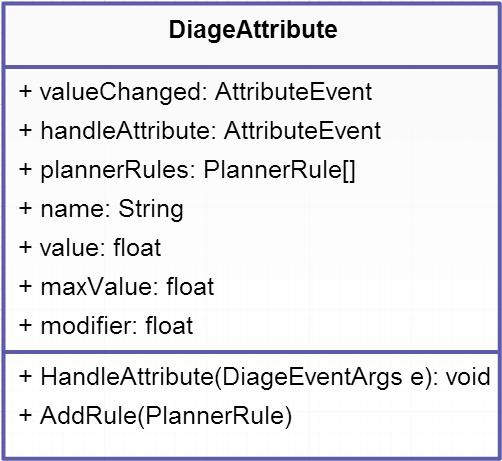
\includegraphics[scale=.7]{attributeUML}
 \caption{Class description of the DiageAttribute}\label{fig:attributeUML}
\end{figure}
\begin{figure}[p]
	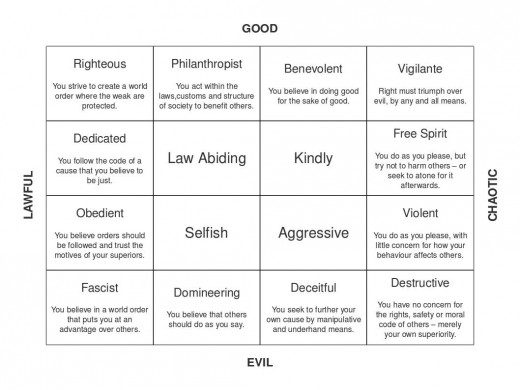
\includegraphics[scale=.8]{alignment}
	\caption{\textit{Dungeons \& Dragons} alignment sheet}\label{fig:dnd}
\end{figure}

%\section{The Narrator}
%\textit{The Narrator} is the both the narrative planning system and overall controller for \diage. This section will give a brief run-down on the components that make up the Narrator.
%First and foremost are the actor attributes that specify how actors should behave in any given situation.
%On first glance these attributes are simple key-value pairs that can be used to describe a myriad of character traits on the actor, making actors behave differently according to what attributes they have.
%When actors act with each other, they do so through their attributes.
%Closely tied with the player character's attributes is the planning tracker. 
%This component tracks the history of the players actions to know how to surprise and/or comfort the player. 
%If a persistent world is used, the narrator keeps a history on all former player characters that lived within that world. 
%When \diage is used in combination with a DML-diagram, the Narrator will distribute all objects described within the diagram throughout the world. If there is no diagram specified the narrator will generate one, and continue with the normal process.
%Lastly there is the narrative planner. The planner takes a look at the current story situation, and decides what will change for the next iteration. 

\section{Initial Generation}
Depending on the input given and the desires of the developer, The narrator does the initial generation of the game world and plots in varying degrees, as seen in algorithm~\ref{alg:initial_setup}.
If no input is given at all, \diage will just generate a random amount of entities to populate the world.
Input can be given either within the game code, or with a DML file (discussed in detail in chapter~\ref{ch:dml}).
Whether specified or not, the player character needs an initial constraint.
This constraint is \his first 'objective'.
This initial constraint can be given within the input, otherwise \diage will take an entity within the world and sets that as player constraint.
Within the algorithm we see a section dedicated to custom rules.
These rules can manipulate anything within the story setting.
As an example I created a rule that randomly sets entities to a space as seen in procedure~\ref{proc:rule_example}.
The given example is purely non-deterministic, but is a simple matter to populate the spaces more evenly with the entities.
This rule system is used throughout \diage as a generalized form to give the developer more control on what a given entity can do.
\begin{algorithm}
	\KwIn{entities; customRules;}
	\KwOut{Initial world state}
	let \textit{entities} be all entities within current world state\;
	let \textit{customRules} be the custom behaviour as specified by the developer\;
	\ForEach{rule in customRules}{
		rule.Invoke();
	}
	\If{entities.count $\leq$ 0}{
		entities = GenerateRandomEntities(\textit{max})\;
	}
	\If{player.constraint == null}{
		\textbf{select random} \textit{e} \textbf{from} \textit{entities}\;
		player.constraint = \textit{e}\;
	}
    \caption{Initial planning}\label{alg:initial_setup}
\end{algorithm}
\begin{procedure}
	\tcc{Populates the spaces with the current entities within world state}
	\KwIn{entities; spaces;}
	\KwOut{All entities are randomly moved to a space}
	let \textit{entities} be all objects within current world state, excluding spaces\;
	let \textit{spaces} be all spaces within current world state\;
	\While{entities.count $>$ 0}{
		\textbf{select random} \textit{s} \textbf{from} \textit{spaces}\;
		entities.pop().MoveToSpace(s)\;
	}
	\caption{PopulateSpaces()}\label{proc:rule_example}
\end{procedure}
\section{Step Generation}
When the initial generation is complete, the player should carry out \his objective.
When the objective has been completed, the planner will automatically start a step generation.
This generation is like the initial generation but uses the actor attribute system and the player as extra input.
The attribute system will be covered in a later section.
This step generation looks at all the given variables and generates a new constraint for the player (see procedure~\ref{proc:generate_constraint}).
The longer the character's life, the more exact this generation will be; for any action taken by the player can be used in the generation.
\begin{algorithm}
	\KwIn{entities; actors; player; customRules;}
	\KwOut{new world state}
	let \textit{entities} be all entities, excluding actors and the player\;
	let \textit{actors} be all actors, including the player\;
	\ForEach{actor in actors}{
		actor.rules.Invoke()\;
	}
	\tcc{It's possible that one of the rules gave the player a constraint, so we'll check}
	\If{player.constraint == null}{
		GenerateConstraint(player)\;
	}
	\ForEach{rule in customRules}{
		rule.Invoke()\;
	}
	\caption{Step planning}\label{alg:step_planning}
\end{algorithm}
\begin{procedure}
	\KwIn{player}
	\KwOut{new constraint for the player}
		\eIf{rules.count $\geq$ 0}{
			\ForEach{item in rules}{
				rules.invoke(player)\;
			}}{
				\textbf{select random} \textit{e} \textbf{from} \textit{entities}\;
				player.constraint = \textit{e}\;
			}
	\caption{GenerateConstraint(Player)}\label{proc:generate_constraint}
\end{procedure}
\section{Events}
Riedl and Young\cite{Riedl:2004:IPM:1018409.1018753} and Julie Porteous and Marc Cavazza\cite{Porteous:2009:CNG:1695522.1695557} have demonstrated that stories are perfectly suited to be represented as a sequence of temporal and causal events.
Porteous and Cavazza suggest to use events as a constraint for partial temporal order, using operators as seen in figure~\ref{fig:events}.
These operators ensure that we have some control and gives us a partial temporal order, partial because not all of the events are ordered with respect to each other.
The table is further expanded upon in their paper \textit{Controlling Narrative Generation with Planning Trajectories: the Role of Constraints}~\cite{Porteous:2009:CNG:1695522.1695557}. The Narrator uses event constraints like this to layer plots and direct the player on what to do next.
In the context of a \rogue we don't know when the story is going to stop, as it stops with the death of the player character.
That could be within 2 minutes, but it could be several weeks.
\diage takes this into account by keep adding segments onto a story, sometimes using information gained from previous plots and at other times creating entire new spaces and NPCs therein.
So the operators that Porteous uses we use within these small story steps instead of the entire narrative.

\begin{figure}
\begin{tabular}{|l||l|}
\hline 
operator & meaning \\ 
\hline
\hline 
\textit{sometime-before a b} & \textit{b} must be made true for the first time before \textit{a} \\ 
\hline 
\textit{sometime a} & predicate \textit{a} must be true at some stage of the narrative \\ 
\hline 
\textit{at-end a} & predicate \textit{a} must be true at the end of the narrative \\ 
\hline 
\end{tabular} 
\caption{Event constraints as presented by Julie Porteous}\label{fig:events}
\end{figure}

\section{Planning flow}
The previous sections described the processes that \diage goes through when generating a new world.
The flowchart in figure~\ref{fig:diage_flowchart} displays the steps taken by the planner.
The initial generation influences the world by setting up spaces, actors, and objects and manipulating these entities by their specific rules.
After this, the player can, and will, influence the world by acting in it.
The planner keeps track of \his actions and saves this for future story generation \footnote{For example; a foe thought defeated returns for a rematch.}.
The step generation gets activated automatically when the player's constraint is removed, i.e.
a plot is resolved.
This can also be manually activated by the author on whatever occasion or event \he wishes.
After the step generation the player gets \his new constraint and, depending on the generative rules used, the world can be manipulated too.
Be that actors that move, or new spaces that are generated.
The step generation is highly dependant upon the player's attributes, as everything can react to the gain or loss between story steps.
The actor attributes are a powerful tool in the \diage arsenal, and the (game)world literary revolves around them.
It has to be noted, that the design of \diage works with semi-persistent worlds too.
The world data can be saved to be used in a later play-through, giving the world a whole epic of one player, and starting the next.
\begin{figure}[p]
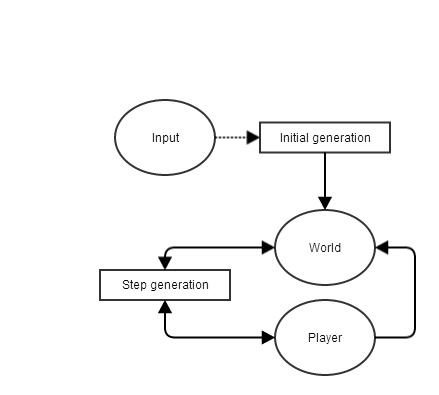
\includegraphics[scale=.8]{diage_planner}
\caption{Simplified Narrator flowchart}\label{fig:diage_flowchart}
\end{figure}

\section{Evaluation}
I wanted a certain control on the narrative of Rouge, and I opted to use a narrative planner to give me those results.
The only sensible evaluation is that a combination of BDI techniques and a narrative planner would be the most favourable, but due to time constraints that would not have worked.
My choice to use a narrative planner was made from the need to have a central system to give commands to.
These commands are now given in the form of the actor attributes, but there is a point to be made that the attributes are easily extended to encompass a BDI framework.
Future work with this system could certainly encompass this change, but I stand by my choice with the time frame I had. 
The narrative planner was needed to convey the author-centric approach that I sought, whereas a bare-bones BDI framework would not.

The narrative planner shines in it's ability to be controlled by very simple constraints.
Simply limiting the exposed attributes can heavily influence the Narrator's decision making.
Another method of control is increasing the Narrator's bias towards certain attributes, so they will be used before any other.
The downside is that, as the Narrator acts as every NPC, the other actors in the story can feel monotone and boring.
In the same vain, the NPCs never act with, or react to, each other.
Everything is focused upon the story of the protagonist, but the world feels empty without him.
The latter part could be resolved by using a more sophisticated AI system, such as a BDI model for NPCs, and letting the actors react to each other, coordinated by the Narrator, to give a more natural feel to the story and the world.